\subsection{RFR File Format}

The RFR file is to restart (i.e. continue) simulations.
It can be produced with help of the RF2TP converter (Kunz 2002).
The RFR file contains 3 blocks: data control, data definition and data area.

\vspace{5mm}
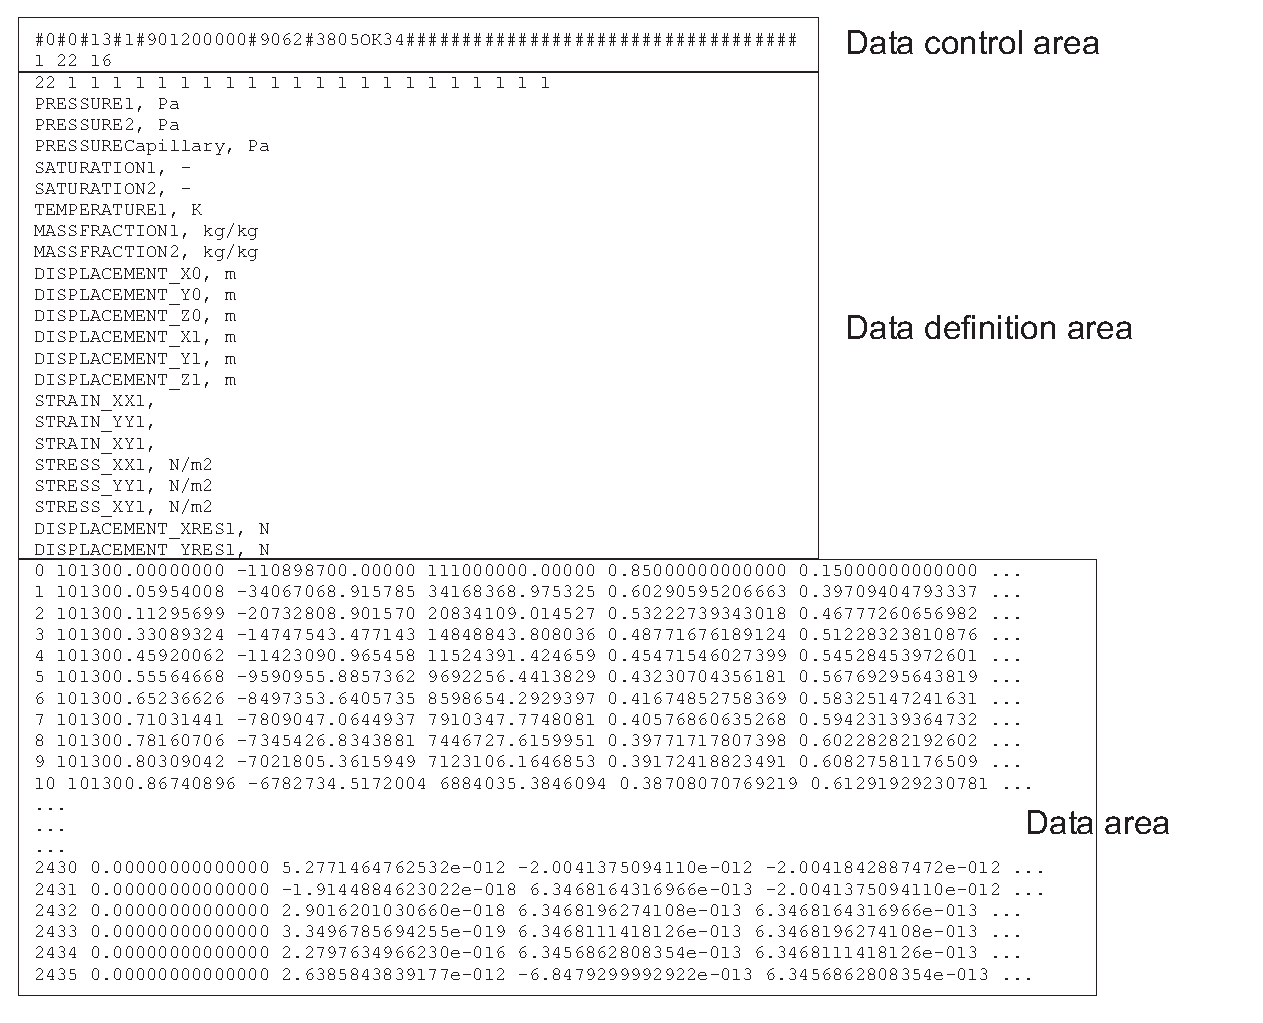
\includegraphics[width=1.0\columnwidth]{figures/rfrfile.eps}  % Filename.eps


\subsubsection{Data control area}

The parameters of the head line are separated by double-crosses.

\footnotesize
\hrule
\begin{minipage}[t]{4cm}
Variable name
\begin{verbatim}
rfr_file->art
rfr_file->bin
nr
rfr_file->geom
startzeit
rfr_file->zeitschritt
rf_filetype
rfr_mesh_doesnt_fit_data
\end{verbatim}
\end{minipage}
%
\begin{minipage}[t]{4cm}
Parameter meaning
\begin{verbatim}
0: has to be zero
0: ASCII format
13:
1:
901200000: beginning from this time the simulation is continued
9062: time step number of previous simualtion
3805OK34: RF/RM version number
\end{verbatim}
\end{minipage}
\hrule
\normalsize

\bigskip
The parameters of the second line are as follows.

\footnotesize
\hrule
\begin{minipage}[t]{4cm}
Variable name
\begin{verbatim}
dateityp
anz_n
anz_e
rfr_nodes
rfr_elements
\end{verbatim}
\end{minipage}
%
\begin{minipage}[t]{4cm}
Parameter meaning
\begin{verbatim}
1:
22: 22 node values are written
16: 16 element values are written
\end{verbatim}
\end{minipage}
\hrule
\normalsize


\subsubsection{Data definition area}

The first line of the data definition area gives the number of model node values
to output an their vector type.

\footnotesize
\hrule
\begin{minipage}[t]{4cm}
Variable name
\begin{verbatim}
\end{verbatim}
\end{minipage}
%
\begin{minipage}[t]{4cm}
Parameter meaning
\begin{verbatim}
22: number of node values to output
1: vector type of node value (scalar: 1 component)
...
\end{verbatim}
\end{minipage}
\hrule
\normalsize

\bigskip
It follows the definition of all node quantities: name and unit

\footnotesize
\hrule
\begin{minipage}[t]{4cm}
Variable name
\begin{verbatim}
PRESSURE1, Pa
\end{verbatim}
\end{minipage}
%
\begin{minipage}[t]{4cm}
Parameter meaning
\begin{verbatim}
quantity name, quantity unit
\end{verbatim}
\end{minipage}
\hrule
\normalsize

\bigskip
The data definition area can be configured by a RF/RM model.
Only those model node data will be written for which the parameter \texttt{save} is set.

\footnotesize
\begin{verbatim}
in mod_xxxx.c
void MODConfigNODValues_XXXX(void)
{
  save=1;
  ModelsAddNodeValInfoStructure("PRESSURE1","Pa",save, 0, 1, 1, 0.);
}
\end{verbatim}
\normalsize



\subsubsection{Data area}

The data area is simply a table of the specified node values.

\footnotesize
\hrule
\begin{minipage}[t]{4cm}
\begin{verbatim}
NODE1 QUANTITY1 QUANTITY2 QUANTITY3 QUANTITY4 ...
NODE2 QUANTITY1 QUANTITY2 QUANTITY3 QUANTITY4 ...
NODE3 QUANTITY1 QUANTITY2 QUANTITY3 QUANTITY4 ...
...

\end{verbatim}
\end{minipage}
\hrule
\normalsize

\vfill \LastModified{OK 21.07.2003}
